\chapter{Implementation and Results}
\label{chap:implementation-results}

\section{System Overview}

\SystemName{} is implemented as a Python 3.11 package, FastAPI application,
React frontend, PostgreSQL/pgVector database, and background worker. The
architecture in \Cref{fig:overall-architecture} separates application,
orchestration, knowledge processing, model, evaluation, governance, agent,
prompt-engineering, and storage responsibilities.

\begin{landscape}
  \begin{figure}[p]
    \centering
    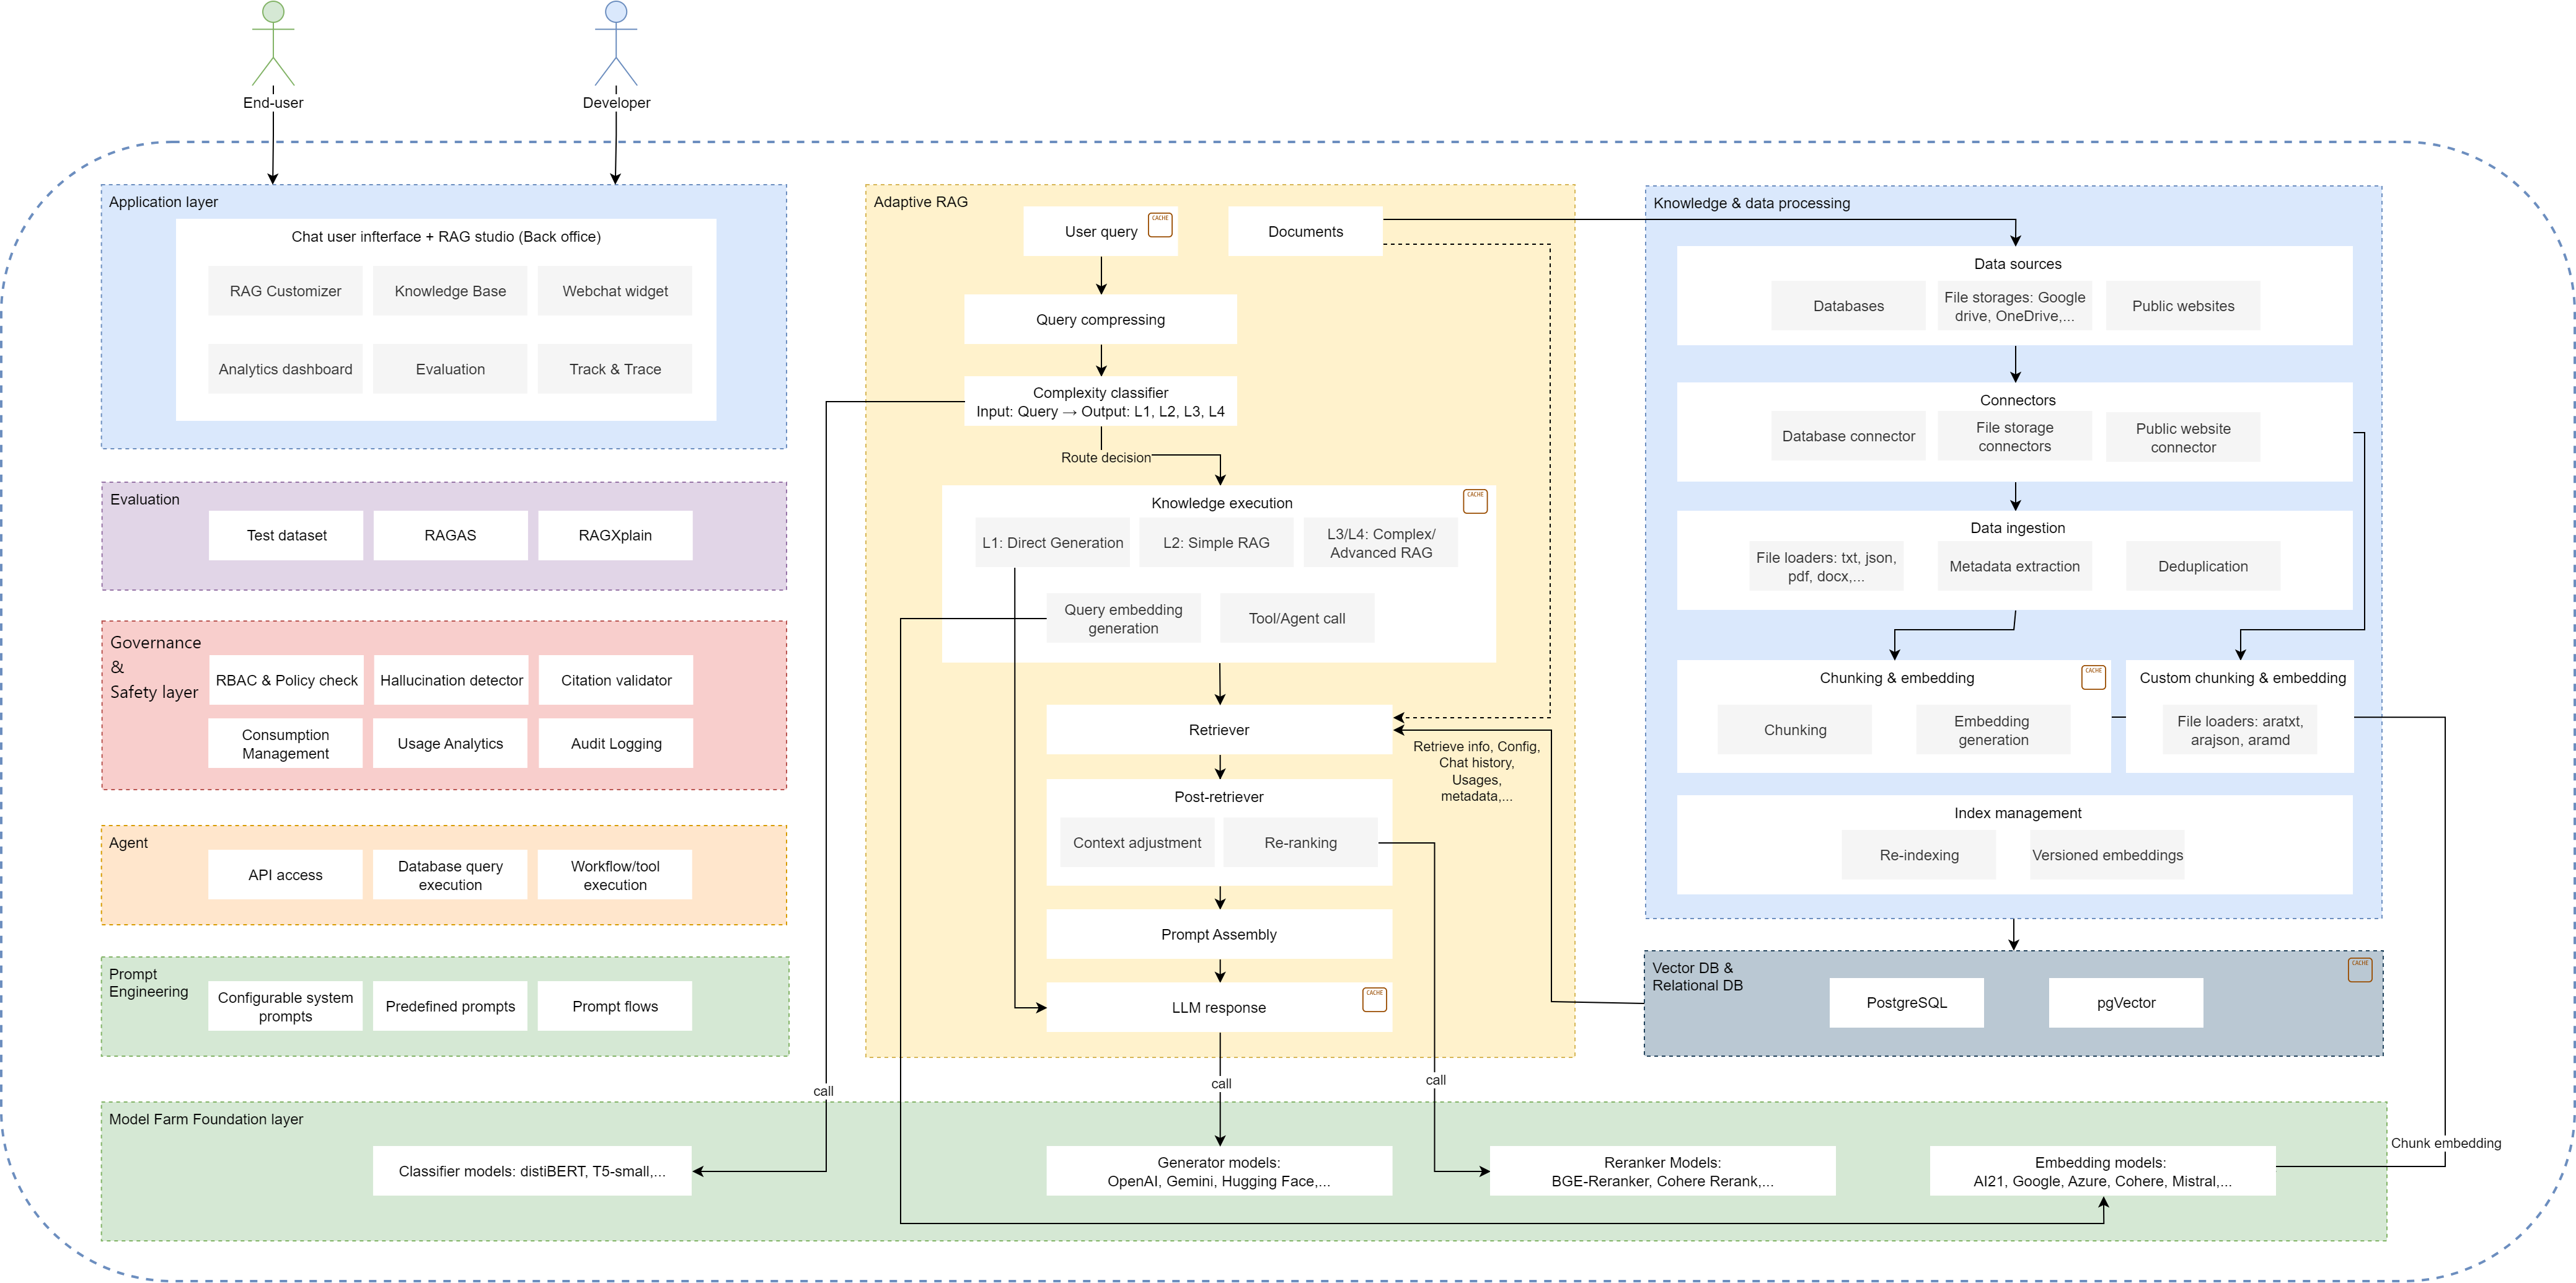
\includegraphics[width=0.98\linewidth,height=0.82\textheight,keepaspectratio]{figures/architecture_landscape.png}
    \caption{Implemented layered architecture of the \SystemName{} system.}
    \label{fig:overall-architecture}
  \end{figure}
\end{landscape}

The separation is behavioral rather than cosmetic. Knowledge ingestion can be
tested without running the React UI. The answer service can use a JSON
repository for bounded tests or PostgreSQL for the full system. Model providers
are selected by deployment ID rather than imported directly into RAG logic.
Evaluation calls the same answer orchestration used by chat, avoiding a
parallel benchmark-only implementation.

\section{Application and API Layer}

The React studio provides Main, Knowledge Bases, AI Models, Evaluation, and
Analytics screens under an authenticated top navigation. FastAPI validates
requests, resolves the current user and role, enforces resource policies, and
returns synchronous JSON or SSE. JWT-backed local users have \texttt{admin} or
\texttt{user} roles. AI Models and organization-wide analytics are restricted
to administrators, while authenticated users can chat and submit feedback.

The Main screen uses three resizable panels:

\begin{enumerate}
  \item an Explorer with New Chat, search, pinned Library, and recent
  conversations;
  \item the chat panel with persistent messages, document filtering, streaming,
  citations, sources, traces, feedback, answer versions, Stop, Retry, and
  Regenerate; and
  \item the RAG Customizer with Knowledge Base status, General settings,
  Adaptive RAG controls, and generator/prompt controls.
\end{enumerate}

Panel widths and collapsed state persist in browser storage. Conversation
history, configuration snapshots, contexts, trace IDs, message states, and
answer versions persist on the server. This means restoring a chat also
restores source links, citation warnings, follow-up-rewrite markers, and trace
navigation.

\ReportAsset{ui-main.png}{Main screen with Explorer, streaming chat, and RAG Customizer.}{fig:ui-main}

\section{Knowledge Base Implementation}

The Knowledge Bases screen manages a one-to-many relationship between a
knowledge base and its documents. A shared Add/Modify dialog captures name,
description, source, chunking profile, embedding deployment, and external
processing policy. Documents are browsed with server-side search and
pagination. Expanding a document lazily loads its chunks and displays metadata,
embedding identity, and processing trace.

Local upload and prepared WixQA import are operational. Public websites use the
safety policy described in \Cref{chap:methodology}. Google Drive, OneDrive, and
database sources are visible extension points but unavailable. Prepared WixQA
import can select a deterministic document count rather than requiring the
entire corpus. Evaluation compatibility records the selected source IDs so a
benchmark can sample only cases grounded in those documents.

Ingestion, re-indexing, and corpus import are durable jobs. The worker claims
leased jobs with PostgreSQL locking, updates bounded progress stages, and
checks cancellation between batches. Uploads are staged by content hash.
Unchanged chunks can reuse embeddings. A failed draft does not replace the
active index.

\ReportAsset{ui-knowledge-bases.png}{Knowledge Base management, paginated documents, and processing details.}{fig:ui-knowledge}

\section{AI Models and Model Gateway}

AI Models presents deployments as smaller grouped cards under Experimentation,
Production Direct, and Local. A single consistent-width wizard selects a
provider or local model, captures connection details, tests the endpoint, saves
it, then creates and enables a deployment. Editing uses the same flow.

Connections and deployments are separate database entities. For example, one
OpenRouter connection may support several deployments with different
provider-native model IDs and capabilities. Stored model IDs are normalized at
runtime:

\begin{table}[H]
  \centering
  \caption{Representative runtime model-ID mapping.}
  \label{tab:model-id-mapping}
  \begin{tabularx}{\textwidth}{p{0.2\textwidth}p{0.34\textwidth}X}
    \toprule
    Connection & Stored model ID & LiteLLM runtime ID\\
    \midrule
    OpenRouter & \texttt{google/gemma-\ldots} & \texttt{openrouter/google/gemma-\ldots}\\
    OpenAI direct & \texttt{gpt-4.1-mini} & \texttt{gpt-4.1-mini}\\
    Gemini direct & \texttt{gemini-2.5-flash} & \texttt{gemini/gemini-2.5-flash}\\
    Ollama & \texttt{llama3.1} & \texttt{ollama\_chat/llama3.1}\\
    vLLM & server model name & \texttt{hosted\_vllm/<model>}\\
    \bottomrule
  \end{tabularx}
\end{table}

The gateway exposes generation, streaming, embedding, reranking,
classification, planning, judging, and health testing. Local built-ins include
extractive generation, FLAN-T5, hash-384 embedding, MiniLM-384, lexical
reranking, and classifier deployments. Remote calls use one LiteLLM boundary.
Credential values are encrypted before storage and redacted from responses,
errors, usage, and traces.

\ReportAsset{ui-ai-models.png}{AI Models catalog and connection/deployment workflow.}{fig:ui-models}

\section{Adaptive RAG Runtime}

The async answer service prepares a request through policy, conversation
context, reformulation, classification, route selection, retrieval, reranking,
context budgeting, prompt assembly, generation, citation validation,
persistence, and telemetry. Synchronous and streaming endpoints reuse these
stages.

\subsection{Runtime-Truthful Configuration}

Every Main-screen Adaptive RAG control is connected to execution:

\begin{itemize}
  \item the selected classifier controls Adaptive routing, with explicit
  configured/actual/fallback metadata;
  \item the selected planner can rewrite follow-ups, decompose L3 queries, and
  drive bounded L4 actions;
  \item the query embedding is inherited from the active KB index and cannot be
  overridden by a stale chat configuration;
  \item BM25 avoids an embedding call; dense and hybrid retrieval use the
  active index deployment;
  \item reranking executes only when enabled and a compatible deployment is
  selected;
  \item citation settings modify the prompt and validation; and
  \item generator, fallbacks, prompts, style, history, and agent limits are
  preserved in configuration and conversation snapshots.
\end{itemize}

This design addresses a common prototype defect where controls are stored as
metadata but do not affect runtime. Trace summaries distinguish what was
configured from what actually executed.

\subsection{Streaming and Answer Lifecycle}

The streaming endpoint sends \texttt{started}, \texttt{trace},
\texttt{sources}, and \texttt{delta} progress events. It terminates with
\texttt{model\_completed}, \texttt{completed}, \texttt{cancelled}, or
\texttt{error}. LiteLLM
providers stream deltas directly. FLAN-T5 uses a background generation thread
and iterator. The deterministic extractive generator emits bounded chunks.

\begin{figure}[H]
  \centering
  \resizebox{\textwidth}{!}{%
  \begin{tikzpicture}[x=2.4cm,y=0.72cm,font=\small]
    \foreach \name/\x in {UI/0,API/1,Orchestrator/2,Gateway/3,Database/4} {
      \node[font=\bfseries] at (\x,0) {\name};
      \draw[aragline] (\x,-0.35) -- (\x,-10.7);
    }
    \draw[aragarrow] (0,-1) -- node[above]{POST /answer/stream} (1,-1);
    \draw[aragarrow] (1,-2) -- node[above]{create pending messages} (4,-2);
    \draw[aragarrow] (1,-3) -- node[above]{prepare query} (2,-3);
    \draw[aragarrow] (1,-4) -- node[above]{started + trace events} (0,-4);
    \draw[aragarrow] (2,-5) -- node[above]{stream deployment} (3,-5);
    \draw[aragarrow] (3,-6) -- node[above]{model deltas} (2,-6);
    \draw[aragarrow] (2,-7) -- node[above]{delta SSE} (0,-7);
    \draw[aragarrow] (2,-8) -- node[above]{persist content, trace, status} (4,-8);
    \draw[aragarrow] (2,-9) -- node[above]{completed/cancelled/error} (1,-9);
    \draw[aragarrow] (1,-10) -- node[above]{terminal SSE payload} (0,-10);
  \end{tikzpicture}}
  \caption{True provider streaming and durable message-state sequence.}
  \label{fig:streaming-sequence}
\end{figure}


Messages and answer versions use pending, streaming, completed, failed, and
cancelled states. Explicit Stop and client disconnect converge on one
cancellation path. A successful regeneration becomes the canonical assistant
message while preserving previous versions. A failed retry retains partial
content and leaves the prior successful canonical answer unchanged.

\section{Retrieval, Sources, and Grounded Citations}

The retriever supports complete active-index BM25, pgVector dense similarity,
and normalized hybrid ranking. Lexical indexes are cached by KB and active
index version with bounded eviction. A document filter indexes or searches only
selected documents. L3 diagnostics retain subquery, retrieval step, original
rank, aggregated rank, and coverage.

Retrieved chunks receive source labels. Markdown rendering converts valid
labels such as \texttt{[S1]} into accessible buttons, except inside code or
existing links. Clicking a citation opens the Source dialog at the stable chunk
identity. Unknown labels remain visually invalid and appear in the citation
validation trace.

The Source dialog has a searchable selectable list and one focused preview.
It shows rank, score, retrieval mode, document, chunk index, embedding model,
and L3/L4 metadata. The Trace dialog can navigate from a retrieval candidate
to the same source preview.

\section{Observability}

Every answer can produce a versioned, strict UTF-8 trace. PostgreSQL stores
searchable metadata while a gzip artifact stores hierarchical spans. Each span
has stable IDs, parent, sequence, category, status, timestamps, duration,
sanitized inputs/outputs, metrics, model usage IDs, warnings, and errors.
Partial traces are persisted at completed-span boundaries, preserving evidence
for failure and cancellation.

\begin{figure}[H]
  \centering
  \begin{tikzpicture}[node distance=7mm and 12mm]
    \node[araglayer,text width=45mm] (trace) {Answer trace\\request, route, total latency, tokens, cost};
    \node[aragbox,text width=40mm,below left=of trace] (prepare) {Preparation spans\\chat input, history, rewrite, classification, route};
    \node[aragbox,text width=40mm,below right=of trace] (execution) {Execution spans\\retrieval, reranking, prompt, model attempts};
    \node[aragbox,text width=34mm,below=of prepare] (retrieval) {Retrieval diagnostics\\raw/normalized scores and ranks};
    \node[aragbox,text width=34mm,below=of execution] (generation) {Generation diagnostics\\messages, usage IDs, finish reason};
    \node[aragbox,text width=45mm,below=16mm of trace,yshift=-32mm] (final) {Finalization spans\\citations, persistence, chat output};

    \draw[aragarrow] (trace) -- (prepare);
    \draw[aragarrow] (trace) -- (execution);
    \draw[aragarrow] (prepare) -- (retrieval);
    \draw[aragarrow] (execution) -- (generation);
    \draw[aragarrow] (retrieval) -- (final);
    \draw[aragarrow] (generation) -- (final);
  \end{tikzpicture}
  \caption{Hierarchical full-fidelity observability trace model.}
  \label{fig:trace-hierarchy}
\end{figure}


The trace UI shows total latency, tokens, cost, route, models, warnings, a
waterfall, and hierarchical stages. The orchestration root appears in the
waterfall but is not numbered as a pipeline step. Step details provide Inputs,
Outputs, Metrics, Model Usage, and Raw JSON tabs. Summary and waterfall regions
can collapse to prioritize the selected detail.

Artifacts exclude API keys, authorization headers, encrypted credentials, and
raw embedding vectors. The default maximum compressed artifact size is 10 MB
and retention is 30 days. Truncated sections remain valid JSON and record the
reason.

\ReportAsset{ui-trace.png}{Full-fidelity Trace report with waterfall and selected-span details.}{fig:ui-trace}

\section{Evaluation and RAGXplain}

The Evaluation screen creates durable configuration-based experiment matrices.
Each selected saved configuration runs exactly once per selected dataset cell.
The UI shows progress, metric cards, route distribution, leaderboard, and
case-level Trace actions. WixQA eligibility detects mismatched corpus subsets
rather than comparing queries against unrelated KB documents.

The RAGXplain adapter exports question, candidate answer, contexts, and ground
truth, then uses the selected Model Farm judge for six semantic metrics. It
validates that semantic score columns and insight summaries exist before
reporting completion. The embedded viewer automatically loads
\texttt{overall\_insights.json}; no manual upload panel is shown in the normal
flow.

\ReportAsset{ui-evaluation.png}{Configuration-based WixQA experiment and selected-run metrics.}{fig:ui-evaluation}
\ReportAsset{ragxplain-insights.png}{Embedded RAGXplain executive summary and action protocols.}{fig:ui-ragxplain}

\section{Analytics and Feedback}

Analytics is an administrator-only PostgreSQL dashboard. Token Statistics
provides date and dimension filters, totals, daily token/cost trends,
breakdowns by model, KB, configuration, and purpose, and paginated usage
events. Detailed Statistics and Feedbacks reports active conversations,
messages, authenticated active users, and ratings. Tables support server
pagination, filters, column resizing, and horizontal scrolling.

Feedback is attached to one assistant answer version per user. The server
derives the KB, configuration, question, answer, and trace rather than trusting
client snapshots. A rating change updates the same record. The feedback table
links to the exact trace when a durable trace ID is available.

\ReportAsset{ui-analytics.png}{Usage, cost, engagement, and structured feedback analytics.}{fig:ui-analytics}

\section{Deployment and Persistence}

Docker Compose defines PostgreSQL/pgVector, migration, API, and worker services.
Alembic versions the schema. PostgreSQL is the primary backend for jobs,
versioned indexes, paid models, chat history, evaluation, analytics, and traces.
JSON repositories remain available for bounded tests. The application requires
Python 3.11 to stabilize the FastAPI, Transformers, Torch, and pgVector stack.

The worker is separate from the API so indexing and evaluation survive API
reloads. Health and progress endpoints let the UI poll jobs without exposing
secret payloads. Transaction retry and reduced runtime DDL address PostgreSQL
deadlocks observed during early development.

\section{Classifier Data and Final Results}

\subsection{Four-Class Dataset Audit}

\begin{table}[H]
  \centering
  \caption{Prepared four-class dataset audit.}
  \label{tab:dataset-audit}
  \begin{tabularx}{\textwidth}{p{0.37\textwidth}X}
    \toprule
    Audit item & Observed result\\
    \midrule
    Total and balance & \PreparedDatasetRecords{} records;
    \PreparedDatasetPerClass{} per class.\\
    Source contribution & \PreparedOfficialExpertRecords{} ExpertWritten,
    \PreparedOfficialSimulatedRecords{} Simulated,
    \PreparedOfficialSyntheticRecords{} official Synthetic, and
    \PreparedTemplateRecords{} template records.\\
    Grouped split & \PreparedTrainRecords{} train and
    \PreparedValidationRecords{} validation records across
    \PreparedSourceGroups{} source groups.\\
    Data-quality checks & No duplicate IDs, duplicate question groups,
    conflicting question labels, missing classes, or source leakage.\\
    Status & Final DistilBERT and T5-small artifacts trained and evaluated on
    the same grouped validation split.\\
    \bottomrule
  \end{tabularx}
\end{table}

\subsection{Final Four-Class Classifier Comparison}

The final metrics are read from the exported DistilBERT and T5-small metric
artifacts. Both models used the same \FinalClassifierValidationRecords-record
source-grouped validation split, label order, and seed.

\begin{table}[H]
  \centering
  \caption{Final four-class classifier validation results.}
  \label{tab:final-classifier}
  \begin{tabularx}{\textwidth}{p{0.38\textwidth}X X}
    \toprule
    Metric & DistilBERT & T5-small\\
    \midrule
    Accuracy & \FinalDistilBERTAccuracy & \FinalTFiveAccuracy\\
    Macro F1 & \FinalDistilBERTMacroFOne & \FinalTFiveMacroFOne\\
    Advanced precision & \FinalDistilBERTAdvancedPrecision & \FinalTFiveAdvancedPrecision\\
    Advanced recall & \FinalDistilBERTAdvancedRecall & \FinalTFiveAdvancedRecall\\
    Advanced F1 & \FinalDistilBERTAdvancedFOne & \FinalTFiveAdvancedFOne\\
    Complex recall & \FinalComplexRecall & \FinalComplexRecall\\
    Expected calibration error & \FinalDistilBERTECE & \FinalTFiveECE\\
    Average prediction latency & \FinalDistilBERTLatency & \FinalTFiveLatency\\
    Under-routing rate & \FinalUnderRouting & \FinalUnderRouting\\
    Over-routing rate & \FinalOverRouting & \FinalOverRouting\\
    Route-cost regret & \FinalRoutingCostRegret & \FinalRoutingCostRegret\\
    \bottomrule
  \end{tabularx}
\end{table}

Both models produced the same confusion matrix. The only errors were
\FinalClassifierErrors{} complex questions predicted as moderate.

\begin{table}[H]
  \centering
  \caption{Shared final four-class confusion matrix.}
  \label{tab:final-classifier-confusion}
  \begin{tabular}{lrrrr}
    \toprule
    Actual label & Pred. simple & Pred. moderate & Pred. complex & Pred. advanced\\
    \midrule
    Simple & 120 & 0 & 0 & 0\\
    Moderate & 0 & 119 & 0 & 0\\
    Complex & 0 & 6 & 113 & 0\\
    Advanced & 0 & 0 & 0 & 123\\
    \bottomrule
  \end{tabular}
\end{table}

The models are tied on predictive quality. DistilBERT offers the stronger
latency trade-off, while T5-small has the lower calibration error. This makes
DistilBERT the practical default for interactive routing and T5-small a useful
comparison model when calibrated confidence is prioritized.

\section{Primary Configuration Experiment}

The primary completed experiment is \textit{\PrimaryExperimentName}
(\Code{\PrimaryExperimentID}) at Git commit
\Code{\PrimaryExperimentCommit}. It evaluated four saved configurations over
\PrimaryExperimentCases{} compatible questions against a
\PrimaryExperimentKBDocuments-document WixQA Corpus 100 knowledge base. The
sample contained \PrimarySimulatedCases{} Simulated,
\PrimarySyntheticCases{} Synthetic, and \PrimaryExpertCases{} ExpertWritten
cases. Each configuration evaluated the same case IDs with seed
\PrimaryExperimentSeed{} and conversation context disabled.

\begin{table}[H]
  \centering
  \caption{Configuration snapshots in the primary experiment.}
  \label{tab:primary-configurations}
  \small
  \begin{tabularx}{\textwidth}{p{0.19\textwidth}p{0.13\textwidth}p{0.22\textwidth}p{0.08\textwidth}X}
    \toprule
    Configuration & Route & Classifier & Top-\textit{k} & Generator\\
    \midrule
    Adaptive with DistilBERT & Adaptive & DistilBERT v2 & 2 & OpenAI GPT-4.1-mini\\
    Adaptive with T5-small & Adaptive & T5-small v2 & 1 & OpenAI GPT-4.1-mini\\
    Fixed L2 & L2 & Not used & 2 & OpenAI GPT-4.1-mini\\
    Fixed L3 & L3 & Not used & 1 & Local extractive\\
    \bottomrule
  \end{tabularx}
\end{table}

All configurations used hybrid retrieval with reranking disabled and citations
enabled. Quality scores use an equal-dataset macro average so the larger
Synthetic subset does not dominate. The composite weights are 0.30 factuality,
0.30 context recall, 0.15 ROUGE-1, 0.10 ROUGE-2, 0.10 token F1, and 0.05 BLEU.

\begin{table}[H]
  \centering
  \caption{Primary experiment leaderboard.}
  \label{tab:primary-leaderboard}
  \begin{tabularx}{\textwidth}{rXrrr}
    \toprule
    Rank & Configuration & Quality & Avg. latency/case & Avg. cost/case\\
    \midrule
    1 & Adaptive with DistilBERT & \DistilConfigQuality & \DistilConfigLatency & \DistilConfigCost\\
    2 & Fixed L2 & \LTwoConfigQuality & \LTwoConfigLatency & \LTwoConfigCost\\
    3 & Adaptive with T5-small & \TFiveConfigQuality & \TFiveConfigLatency & \TFiveConfigCost\\
    4 & Fixed L3 & \LThreeConfigQuality & \LThreeConfigLatency & \LThreeConfigCost\\
    \bottomrule
  \end{tabularx}
\end{table}

\begin{table}[H]
  \centering
  \caption{Per-dataset quality scores in the primary experiment.}
  \label{tab:primary-dataset-scores}
  \begin{tabular}{lrrr}
    \toprule
    Configuration & Simulated & Synthetic & ExpertWritten\\
    \midrule
    Adaptive with DistilBERT & \DistilDatasetScores\\
    Adaptive with T5-small & \TFiveDatasetScores\\
    Fixed L2 & \LTwoDatasetScores\\
    Fixed L3 & \LThreeDatasetScores\\
    \bottomrule
  \end{tabular}
\end{table}

\begin{table}[H]
  \centering
  \caption{Equal-dataset macro standard metrics.}
  \label{tab:primary-standard-metrics}
  \scriptsize
  \begin{tabular}{lrrrrrr}
    \toprule
    Configuration & Token F1 & BLEU & ROUGE-1 & ROUGE-2 & Context recall & Factuality\\
    \midrule
    Adaptive with DistilBERT & \DistilStdMetrics\\
    Adaptive with T5-small & \TFiveStdMetrics\\
    Fixed L2 & \LTwoStdMetrics\\
    Fixed L3 & \LThreeStdMetrics\\
    \bottomrule
  \end{tabular}
\end{table}

The recorded cost includes answer-pipeline execution and WixQA factuality and
context-recall judges. It excludes the RAGXplain diagnosis performed after the
experiment. Both Adaptive configurations routed all twenty cases to L2, so the
experiment does not distinguish L3 or L4 routing behavior. It also does not
isolate classifier effects: their top-\textit{k} values differ, and Fixed L3
uses a different generator. The leaderboard therefore compares complete saved
configurations rather than individual components.

\subsection{RAGXplain Diagnosis}

RAGXplain diagnosis completed for all twelve configuration--dataset runs. The
semantic scores below average cases within each dataset and then macro-average
the three dataset scores.

\begin{table}[H]
  \centering
  \caption{Equal-dataset macro RAGXplain semantic metrics.}
  \label{tab:primary-ragxplain}
  \scriptsize
  \begin{tabular}{lrrrrrr}
    \toprule
    Configuration & Context rel. & Context adh. & Answer rel. & Context recall & Factuality & Grading note\\
    \midrule
    Adaptive with DistilBERT & \DistilRAGXMetrics\\
    Adaptive with T5-small & \TFiveRAGXMetrics\\
    Fixed L2 & \LTwoRAGXMetrics\\
    Fixed L3 & \LThreeRAGXMetrics\\
    \bottomrule
  \end{tabular}
\end{table}

Across all runs, RAGXplain repeatedly identified retrieval breadth, evidence
coverage, and generator grounding as the main constraints. Its recommended
protocol is to compare larger top-\textit{k} values, evaluate reranking, refine
procedural chunking and query expansion, strengthen grounding instructions,
and require complete step-oriented responses. These recommendations map to
implemented Knowledge Base and RAG Customizer fields and define the next
controlled experiment matrix.
